% Options for packages loaded elsewhere
\PassOptionsToPackage{unicode}{hyperref}
\PassOptionsToPackage{hyphens}{url}
%
\documentclass[
]{article}
\author{}
\date{}

\usepackage{amsmath,amssymb}
\usepackage{lmodern}
\usepackage{iftex}
\ifPDFTeX
  \usepackage[T1]{fontenc}
  \usepackage[utf8]{inputenc}
  \usepackage{textcomp} % provide euro and other symbols
\else % if luatex or xetex
  \usepackage{unicode-math}
  \defaultfontfeatures{Scale=MatchLowercase}
  \defaultfontfeatures[\rmfamily]{Ligatures=TeX,Scale=1}
\fi
% Use upquote if available, for straight quotes in verbatim environments
\IfFileExists{upquote.sty}{\usepackage{upquote}}{}
\IfFileExists{microtype.sty}{% use microtype if available
  \usepackage[]{microtype}
  \UseMicrotypeSet[protrusion]{basicmath} % disable protrusion for tt fonts
}{}
\makeatletter
\@ifundefined{KOMAClassName}{% if non-KOMA class
  \IfFileExists{parskip.sty}{%
    \usepackage{parskip}
  }{% else
    \setlength{\parindent}{0pt}
    \setlength{\parskip}{6pt plus 2pt minus 1pt}}
}{% if KOMA class
  \KOMAoptions{parskip=half}}
\makeatother
\usepackage{xcolor}
\IfFileExists{xurl.sty}{\usepackage{xurl}}{} % add URL line breaks if available
\IfFileExists{bookmark.sty}{\usepackage{bookmark}}{\usepackage{hyperref}}
\hypersetup{
  hidelinks,
  pdfcreator={LaTeX via pandoc}}
\urlstyle{same} % disable monospaced font for URLs
\usepackage[a4paper, left=3cm,right=3cm,top=3cm,bottom=3cm,
headsep=1.5cm]{geometry}
\usepackage{longtable,booktabs,array}
\usepackage{calc} % for calculating minipage widths
% Correct order of tables after \paragraph or \subparagraph
\usepackage{etoolbox}
\makeatletter
\patchcmd\longtable{\par}{\if@noskipsec\mbox{}\fi\par}{}{}
\makeatother
% Allow footnotes in longtable head/foot
\IfFileExists{footnotehyper.sty}{\usepackage{footnotehyper}}{\usepackage{footnote}}
\makesavenoteenv{longtable}
\usepackage{graphicx}
\makeatletter
\def\maxwidth{\ifdim\Gin@nat@width>\linewidth\linewidth\else\Gin@nat@width\fi}
\def\maxheight{\ifdim\Gin@nat@height>\textheight\textheight\else\Gin@nat@height\fi}
\makeatother
% Scale images if necessary, so that they will not overflow the page
% margins by default, and it is still possible to overwrite the defaults
% using explicit options in \includegraphics[width, height, ...]{}
\setkeys{Gin}{width=\maxwidth,height=\maxheight,keepaspectratio}
% Set default figure placement to htbp
\makeatletter
\def\fps@figure{htbp}
\makeatother
\setlength{\emergencystretch}{3em} % prevent overfull lines
\providecommand{\tightlist}{%
  \setlength{\itemsep}{0pt}\setlength{\parskip}{0pt}}
\setcounter{secnumdepth}{-\maxdimen} % remove section numbering
\usepackage{fancyhdr}
\pagestyle{fancy}
\fancyhead[L]{Grupo 2 \\ Cáceres (96454) - del Mazo (100029) \\ Pastine (100017) - Pistillo (99177) }
\fancyhead[R]{71.14 // 91.04 \\ Modelos y Optimización I \\ 2021C1}

\usepackage{listings}
\lstset{
    breaklines=true,
    breakatwhitespace=true,
    basicstyle=\ttfamily\footnotesize,
    frame=l,
    framesep=12pt,
    xleftmargin=12pt,
}
\ifLuaTeX
  \usepackage{selnolig}  % disable illegal ligatures
\fi

\begin{document}

\hypertarget{enunciado---primera-parte}{%
\section{Enunciado - Primera Parte}\label{enunciado---primera-parte}}

Una refinería mezcla 5 tipos de gasolina cruda (Tipo 1, Tipo 2, Tipo 3,
Tipo 4 y Tipo 5) para producir dos tipos de nafta para autos (común y
súper).

La tabla muestra el número de barriles disponibles por día de cada tipo
de gasolina cruda, la potencia de performance y el costo por barril.

\begin{longtable}[]{@{}cccc@{}}
\toprule
Gasolina cruda & Potencia & Barriles / día & Costo / barril \\
\midrule
\endhead
Tipo 1 & 70 & 2000 & 0.8 \\
Tipo 2 & 80 & 4000 & 0.9 \\
Tipo 3 & 85 & 4000 & 0.95 \\
Tipo 4 & 90 & 5000 & 1.15 \\
Tipo 5 & 99 & 3000 & 2 \\
\bottomrule
\end{longtable}

La nafta común debe tener una potencia de al menos 85 y la súper de al
menos 95.

Los contratos de la refinería requieren que al menos se produzcan 8000
barriles por día de nafta súper.

El precio de venta es de \$3.75 por barril de nafta súper y de \$2.85
por barril de nafta común.

¿Qué es lo mejor que se puede hacer con la información disponible?

\begin{enumerate}
\def\labelenumi{\arabic{enumi}.}
\item
  Redactar objetivo, hipótesis, plantear modelo por PLC y realizar una
  corrida con software.
\item
  Hacer un análisis detallado post optimal de la corrida del punto 1.
\end{enumerate}

\hypertarget{enunciado---segunda-parte}{%
\section{Enunciado - Segunda Parte}\label{enunciado---segunda-parte}}

Dada la imposibilidad de cumplir con los contratos se decidió no
realizarlos y re negociar las condiciones. Bajo este nuevo escenario se
pide, realizando independientemente un punto del otro:

\begin{enumerate}
\def\labelenumi{\arabic{enumi}.}
\item
  El sector de ventas nos pide un análisis detallado de los precios de
  venta por barril de nafta súper y nafta común. Ofreciéndoles
  alternativas y explicándoles el porqué de las mismas.
\item
  El sector de compras nos informa que pueden re negociar los precios a
  pagar por los barriles de gasolina cruda, que les gustaría saber qué
  tipos de gasolina (1, 2, 3, 4, 5) nos resultan más estratégicos, que
  precios consideramos más competitivos y que disponibilidades de dichas
  gasolinas crudas nos interesan mantener y/o incrementar.
\item
  El laboratorio de la refinería nos informa que están investigando unos
  nuevos aditivos que les permite incrementar la potencia de las
  gasolinas crudas, nos solicitan les informemos que gasolinas crudas y
  sus respectivas potencias nos interesaría que les demos prioridad en
  las investigaciones.
\end{enumerate}

\newpage

\hypertarget{trabajo-pruxe1ctico---primera-parte}{%
\section{Trabajo Práctico - Primera
Parte}\label{trabajo-pruxe1ctico---primera-parte}}

\hypertarget{situacion-problemuxe1tica}{%
\subsection{Situacion Problemática}\label{situacion-problemuxe1tica}}

Se trata de un problema de planificación de la producción con la
particularidad de que se tienen mezclas de distintos tipos de gasolinas
para producir 2 tipos de nafta como resultado.

Cada mezcla debe cumplir con un mínimo de potencia y se tiene una
demanda mínima de barriles de nafta súper. También en la producción de
la nafta se debe tener en cuenta el costo de cada tipo de combustible.

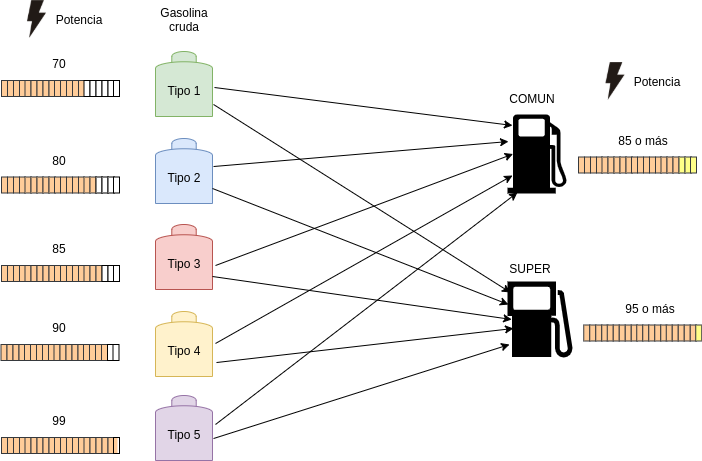
\includegraphics{img/nafta.png}

\hypertarget{objetivo}{%
\subsection{Objetivo}\label{objetivo}}

Determinar la cantidad de los dos tipos de nafta a producir en un día
para maximizar las ganancias totales.

\hypertarget{hipuxf3tesis-y-supuestos}{%
\subsection{Hipótesis y Supuestos}\label{hipuxf3tesis-y-supuestos}}

\begin{itemize}
\tightlist
\item
  Las masas de las gasolinas son aditivas y lineales. Es decir, la
  cantidad final de barriles producidos en cada nafta es igual a la suma
  de las cantidades de barriles de las gasolinas que las componen.
\item
  Se pueden producir cantidades arbitrariamente pequeñas de nafta.
\item
  No es necesario mezclar todos los tipos de gasolina para producir un
  tipo de nafta. Es decir, puede no llegar a utilizarse algún tipo de
  gasolina para algún tipo de nafta y hasta puede ocurrir que la nafta
  esté compuesta por un solo tipo de gasolina.
\item
  Las potencias son una combinación lineal de las potencias de los
  combustibles que componen a la nafta resultante.
\item
  No se pierde volumen al mezclar la gasolina cruda
\item
  No hay pérdidas de barriles en el proceso
\item
  Los precios no varían en el periodo analizado
\item
  No hay más costos que el de los barriles
\item
  Toda la nafta producida va a venderse. No hay stock inicial ni final.
\item
  El consumo de los recursos es directamente proporcional a la cantidad
  fabricada. No importan las proporciones finales de cada nafta mientras
  cumpla con las especificaciones. El resultado y su costo por barril no
  se verá afectado.
\item
  Todos los barriles de gasolina no utilizados se desechan de un período
  a otro.
\item
  Las constantes del modelo no varían.
\item
  El período alcanza para producir tantos barriles de cada tipo de nafta
  como sea necesario.
\item
  No hay materia prima ni productos defectuosos.
\item
  Se pueden usar fracciones de barriles para la produccion de nafta, en
  vez de dedicar un barril entero para cada barril de nafta producido.
\end{itemize}

\hypertarget{identificaciuxf3n-de-variables-de-decisiuxf3n-controlables}{%
\subsection{Identificación de variables de decisión
controlables}\label{identificaciuxf3n-de-variables-de-decisiuxf3n-controlables}}

\(G_{i,k} \: (i \in \{ 1,2,3,4,5 \} \wedge k \in \{C,S\} ) \: [barriles/día]:\)
Gasolina de tipo \(i\) destinada a producir nafta del tipo \(k\) (\(C\)
por común, \(S\) por super)

\(N_k \: (k \in {C,S} ) \: [barriles/día]:\) Nafta de tipo \(k\)
producida\\

La nafta se obtiene de la mezcla de 5 tipos de gasolina
\[N_C = \sum_{i = 1}^{5} G_{i,C}\] \[N_S = \sum_{i = 1}^{5} G_{i,S}\]

\hypertarget{restricciones}{%
\subsection{Restricciones}\label{restricciones}}

Límites de barriles diarios \[G_{1,C}+G_{1,S} \leq 2000\]
\[G_{2,C}+G_{2,S} \leq 4000\] \[G_{3,C}+G_{3,S} \leq 4000\]
\[G_{4,C}+G_{4,S} \leq 5000\] \[G_{5,C}+G_{5,S} \leq 3000\]

Se requieren al menos 8000 barriles de nafta súper \[N_S \geq 8000\]

La nafta común debe tener una potencia de al menos 85
\[G_{1,C} * 70 + G_{2,C} * 80 + G_{3,C} * 85 + G_{4,C} * 90 + G_{5,C}* 99 \geq N_C * 85\]

La nafta súper debe tener una potencia de al menos 95
\[G_{1,S} * 70 + G_{2,S} * 80 + G_{3,S} * 85 + G_{4,S} * 90 + G_{5,S}* 99 \geq N_S * 95\]

\hypertarget{funciuxf3n-objetivo}{%
\subsection{Función Objetivo}\label{funciuxf3n-objetivo}}

\[
Ganancias = 2.85 * N_C + 3.75 * N_S
\]

\[
Costos =
0.8 * (G_{1,C} + G_{1,S}) +  0.9 * (G_{2,C} + G_{2,S}) + 0.95 * (G_{3,C} + G_{3,S}) +
1.15 * (G_{4,C} + G_{4,S}) + 2 * (G_{5,C} + G_{5,S})
\]

\[ Max Z = Ganancias - Costos \]

\hypertarget{soluciuxf3n-y-anuxe1lisis-post-optimal}{%
\subsection{Solución y Análisis Post
Optimal}\label{soluciuxf3n-y-anuxe1lisis-post-optimal}}

Como se puede ver en el anexo, la corrida de \texttt{GLPK} devuelve que
no hay solución optima para las restricciones dadas, y por ende el
problema es incompatible. Analizando el problema, buscamos por el
absurdo el contraejemplo que demuestre que, efectivamente, no hay
semejante solucion:

\begin{quote}
Se quieren producir 8000 barriles de nafta super, con una potencia de al
menos 95. Pero, si tomamos los 5000 barriles de gasolina cruda de tipo
4, y los 3000 barriles de gasolina cruda de tipo 5, mientras que su suma
sí daría 8000 barriles, la combinación de potencia será de 93.375.
\end{quote}

Por supuesto que tomar cualquier otra combinación de gasolinas crudas
devolvería una potencia aun menor que la generada por la solucion
propuesta, considerando que las gasolinas de tipo 4 y 5 son las de mayor
potencia.

Habiendo demostrado que no hay solución óptima, solo nos queda
preguntarnos como subsanar los conflictos de las restricciones dadas.

Las modificaciones que se pueden hacer para llegar a una solución que
cumpla con lo pedido puede ser cualquiera de las siguientes opciones, o
bien una combinación adecuada de todos los puntos listados:

\begin{itemize}
\item
  Se deben producir menos barriles de nafta super por día, en vez de
  8000

  \begin{itemize}
  \tightlist
  \item
    Al producir 5000 barriles provenientes de 3000 de gasolina de tipo 5
    y 2000 de gasolina de tipo 4, se llega a una potencia de nafta super
    de 95.4
  \end{itemize}
\item
  Se debe conseguir un nuevo tipo de gasolina cruda, de mayor potencia
  que la gasolina de tipo 5, procurando que haya los suficientes
  barriles para llegar a los 8000 por día de nafta super

  \begin{itemize}
  \tightlist
  \item
    Al combinar 3000 barriles de una gasolina cruda hipotética de tipo 6
    que tenga una potencia de 104, con los 5000 barriles de tipo 4, se
    consiguen 8000 barriles de nafta super de 95.25 de potencia
  \end{itemize}
\item
  Se debe aumentar la cantidad de barriles de gasolina de tipo 5 de tal
  manera que se cumpla la restricción de 8000 barriles diarios

  \begin{itemize}
  \item
    Se pueden usar 8000 barriles de tipo 5
  \item
    Se pueden usar unos 3500 barriles de tipo 4, y 4500 de tipo 5, así
    llegando a una potencia de 95.0625
  \end{itemize}
\item
  Se debe producir nafta super con menor potencia a 95

  \begin{itemize}
  \tightlist
  \item
    Se puede buscar una potencia de al menos 93
  \end{itemize}
\end{itemize}

Tomando por supuesto que la restricción de producir al menos 8000
barriles de nafta super por día es la más restrictiva (valga la
redundancia) de todas las conflictivas, y que es la más facil de
subsanar, se puede hacer una corrida del modelo sin esta restricción,
llegando así a una solución optima: generar \$32080 de ganancias,
produciendo 16300 barriles de nafta comun y 1700 de nafta super. Las
especificaciones de esta corrida estan presentes en el anexo de este
informe.

\newpage

\hypertarget{software-tp.mod}{%
\subsection{\texorpdfstring{Software:
\texttt{TP.mod}}{Software: TP.mod}}\label{software-tp.mod}}

\lstinputlisting{TP.mod}

\newpage

\hypertarget{soluciuxf3n-con-glpk-tp.sol}{%
\subsection{\texorpdfstring{Solución con \texttt{GLPK}:
\texttt{TP.sol}}{Solución con GLPK: TP.sol}}\label{soluciuxf3n-con-glpk-tp.sol}}

\lstinputlisting{TP.sol}

\newpage

\hypertarget{soluciuxf3n-con-glpk-sin-la-restricciuxf3n-de-producir-8000-barriles-de-nafta-super-tp-mod.sol}{%
\subsection{\texorpdfstring{Solución con \texttt{GLPK} sin la
restricción de producir 8000 barriles de nafta super:
\texttt{TP-mod.sol}}{Solución con GLPK sin la restricción de producir 8000 barriles de nafta super: TP-mod.sol}}\label{soluciuxf3n-con-glpk-sin-la-restricciuxf3n-de-producir-8000-barriles-de-nafta-super-tp-mod.sol}}

\lstinputlisting{TP-mod.sol}

\newpage

\hypertarget{trabajo-pruxe1ctico---segunda-parte}{%
\section{Trabajo Práctico - Segunda
Parte}\label{trabajo-pruxe1ctico---segunda-parte}}

\hypertarget{modelado-y-resultados-en-lindo}{%
\subsection{Modelado y Resultados en
Lindo}\label{modelado-y-resultados-en-lindo}}

\hypertarget{funcional}{%
\subsubsection{Funcional}\label{funcional}}

\texttt{MAX\ 2.05\ G1C\ +\ 1.95\ G2C\ +\ 1.9\ G3C\ +\ 1.7\ G4C\ +\ 0.85\ G5C\ +\ 2.95\ G1S\ +\ 2.85\ G2S\ +\ 2.8\ G3S\ +\ 2.6\ G4S\ +\ 1.75\ G5S}

\hypertarget{restricciones-1}{%
\subsubsection{Restricciones}\label{restricciones-1}}

\begin{lstlisting}
ST
LimBar1) G1C + G1S <= 2000
LimBar2) G2C + G2S <= 4000
LimBar3) G3C + G3S <= 4000
LimBar4) G4C + G4S <= 5000
LimBar5) G5C + G5S <= 3000
NComun) 70 G1C + 80 G2C + 85 G3C + 90 G4C + 99 G5C - 85 G1C - 85 G2C - 85 G3C - 85 G4C - 85 G5C >= 0
NSuper) 70 G1S + 80 G2S + 85 G3S + 90 G4S + 99 G5S - 95 G1S - 95 G2S - 95 G3S - 95 G4S - 95 G5S >= 0
END
\end{lstlisting}

\hypertarget{resultados}{%
\subsubsection{Resultados}\label{resultados}}

\begin{lstlisting}
LP OPTIMUM FOUND AT STEP 7

OBJECTIVE FUNCTION VALUE

32080.00
\end{lstlisting}

\begin{lstlisting}
VARIABLE VALUE REDUCED COST
G1C 2000.000000 0.000000
G2C 3642.105225 0.000000
G3C 4000.000000 0.000000
G4C 5000.000000 0.000000
G5C 1657.894775 0.000000
G1S 0.000000 0.000000
G2S 357.894745 0.000000
G3S 0.000000 0.000000
G4S 0.000000 0.000000
G5S 1342.105225 0.000000

ROW SLACK OR SURPLUS DUAL PRICES
LIMBAR1) 0.000000 0.700000
LIMBAR2) 0.000000 1.500000
LIMBAR3) 0.000000 1.900000
LIMBAR4) 0.000000 2.150000
LIMBAR5) 0.000000 2.110000
NCOMUN) 0.000000 -0.090000
NSUPER) 0.000000 -0.090000

NO. ITERATIONS= 7

RANGES IN WHICH THE BASIS IS UNCHANGED:

                           OBJ COEFFICIENT RANGES

VARIABLE CURRENT ALLOWABLE ALLOWABLE
COEF INCREASE DECREASE
G1C 2.050000 INFINITY 0.000000
G2C 1.950000 0.000000 1.357143
G3C 1.900000 INFINITY 0.000000
G4C 1.700000 INFINITY 0.000000
G5C 0.850000 0.000000 0.000000
G1S 2.950000 0.000000 INFINITY
G2S 2.850000 2.216666 0.000000
G3S 2.800000 0.000000 INFINITY
G4S 2.600000 0.000000 INFINITY
G5S 1.750000 0.000000 0.000000

                           RIGHTHAND SIDE RANGES
      ROW         CURRENT        ALLOWABLE        ALLOWABLE
                    RHS          INCREASE         DECREASE

LIMBAR1 2000.000000 1133.333252 1400.000000
LIMBAR2 4000.000000 3399.999756 3295.238281
LIMBAR3 4000.000000 INFINITY 4000.000000
LIMBAR4 5000.000000 4200.000000 3399.999756
LIMBAR5 3000.000000 12357.143555 1214.285767
NCOMUN 0.000000 17000.000000 21000.001953
NSUPER 0.000000 4857.143066 49428.574219
\end{lstlisting}

\hypertarget{gruxe1ficos}{%
\subsubsection{Gráficos}\label{gruxe1ficos}}

\hypertarget{curvas-de-oferta-en-funciuxf3n-de-la-ganancia}{%
\paragraph{Curvas de oferta en función de la
ganancia}\label{curvas-de-oferta-en-funciuxf3n-de-la-ganancia}}

\begin{longtable}[]{@{}cc@{}}
\toprule
Nafta Común & Nafta Súper \\
\midrule
\endhead
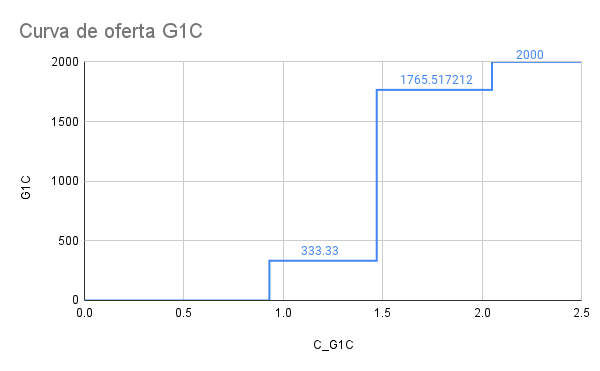
\includegraphics[width=3.125in,height=\textheight]{img/G1C.png} &
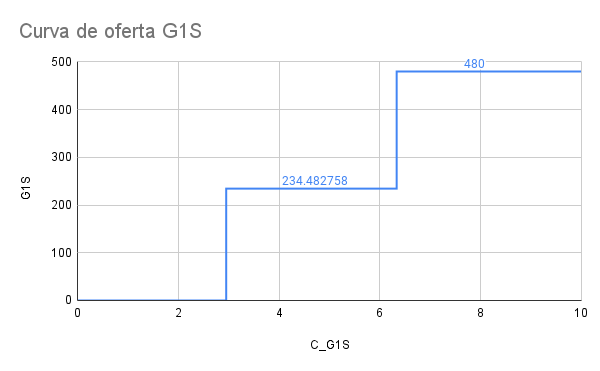
\includegraphics[width=3.125in,height=\textheight]{img/G1S.png} \\
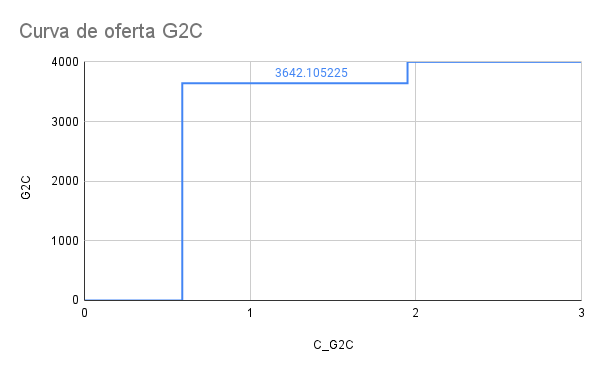
\includegraphics[width=3.125in,height=\textheight]{img/G2C.png} &
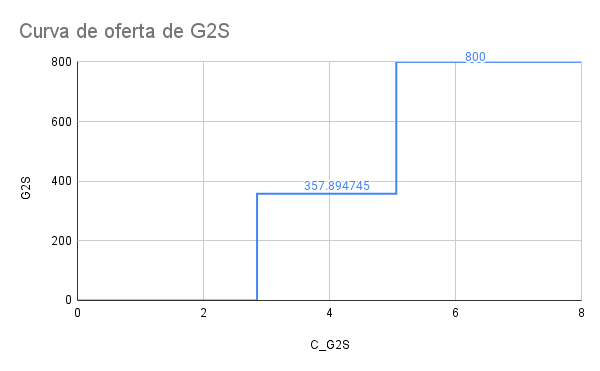
\includegraphics[width=3.125in,height=\textheight]{img/G2S.png} \\
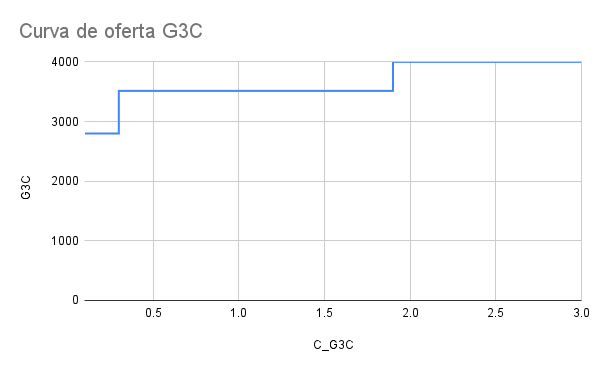
\includegraphics[width=3.125in,height=\textheight]{img/G3C.png} &
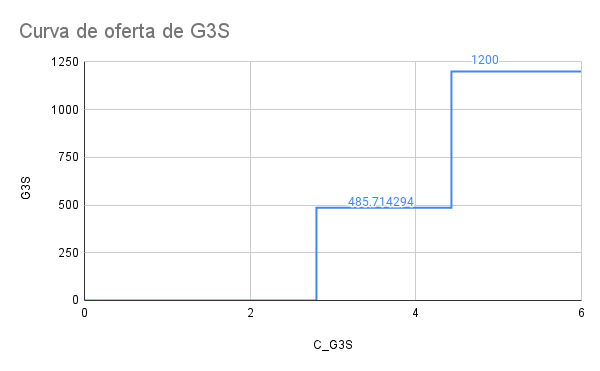
\includegraphics[width=3.125in,height=\textheight]{img/G3S.png} \\
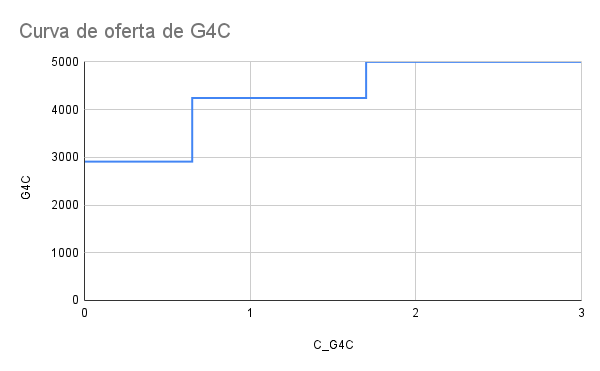
\includegraphics[width=3.125in,height=\textheight]{img/G4C.png} &
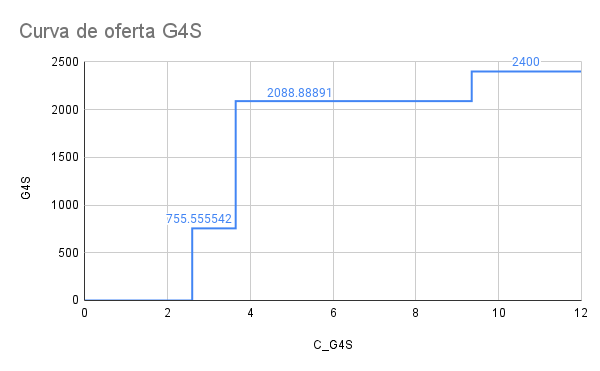
\includegraphics[width=3.125in,height=\textheight]{img/G4S.png} \\
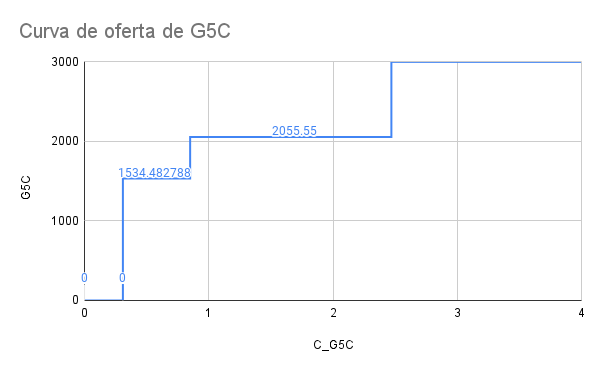
\includegraphics[width=3.125in,height=\textheight]{img/G5C.png} &
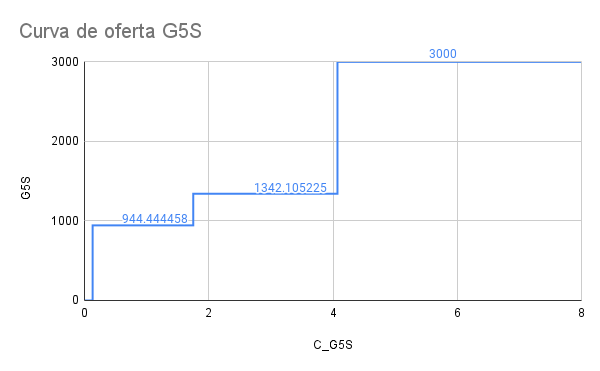
\includegraphics[width=3.125in,height=\textheight]{img/G5S.png} \\
\bottomrule
\end{longtable}

\hypertarget{anuxe1lisis}{%
\subsection{Análisis}\label{anuxe1lisis}}

El precio actual de venta de Nafta Súper es de \$3,75, y en el funcional
se ve reflejado en la parte:

\texttt{\textbackslash{}textbf\{(G1S\ +\ G2S\ +\ G3S\ +\ G4S\ +\ G5S)\ *\ 3,75\}\ -\ 0,8\ *\ G1S\ -\ 0,9\ *\ G2S\ -\ 0.95\ *\ G3S\ -\ 1,15\ *\ G4S\ -\ 2\ *\ G5S\ =\ 2,95\ *\ G1S\ +\ 2,85\ *\ G2S\ +\ 2,8\ *\ G3S\ +\ 2,6\ *\ G4S\ +\ 1,75\ *\ G5S}

En el último término se tienen las constantes
\texttt{Cj\ =\ (2.95\ 2.85\ 2.8\ 2.6\ 1.75} correspondientes a las
ganancias por barril de gasolina de tipo ``j'' destinado a la nafta
súper

En los gráficos de arriba pueden verse las curvas de oferta de cada
barril de gasolina ``j'' destinado a nafta super, variando estas Cj

P\_NC = precio nafta comun P\_NS = precio nafta super

\hypertarget{nafta-de-tipo-1}{%
\subsubsection{Nafta de tipo 1}\label{nafta-de-tipo-1}}

Sabemos que del tipo 1 no vamos a poder producir más de 2000 barriles, y
aumentar el precio de P\_NC no va a cambiar la cantidad de GC1 producida
(ver tabla curva de oferta GC1). Si quisieramos producir menos barriles
GC1 (para no tener al recurso saturado) y producir más barriles GS1,
tendremos que aumentar el P\_NS

\end{document}
